\documentclass[11pt,a4paper]{article}

% ── Packages ──────────────────────────────────────────────────────────
\usepackage[margin=1in]{geometry}
\usepackage{graphicx}
\usepackage{booktabs}
\usepackage{multirow}
\usepackage{amsmath,amssymb}
\usepackage{hyperref}
\usepackage{xcolor}
\usepackage{enumitem}
\usepackage{float}
\usepackage{caption}
\usepackage{subcaption}
\usepackage[numbers]{natbib}
\usepackage{fancyhdr}
\usepackage{titlesec}
\usepackage{parskip}
\usepackage{array}
\usepackage{makecell}

% ── Page style ────────────────────────────────────────────────────────
\pagestyle{fancy}
\fancyhf{}
\rhead{\small ICD-10 Code Prediction from MIMIC-IV}
\lhead{\small NLP Final Project --- Spring 2025}
\cfoot{\thepage}
\renewcommand{\headrulewidth}{0.4pt}

% ── Section formatting ────────────────────────────────────────────────
\titleformat{\section}{\large\bfseries}{\thesection}{1em}{}
\titleformat{\subsection}{\normalsize\bfseries}{\thesubsection}{1em}{}

% ── Hyperlink styling ─────────────────────────────────────────────────
\hypersetup{
    colorlinks=true,
    linkcolor=blue!70!black,
    citecolor=blue!70!black,
    urlcolor=blue!70!black,
}

\begin{document}

% ══════════════════════════════════════════════════════════════════════
% TITLE
% ══════════════════════════════════════════════════════════════════════
\begin{center}
    {\LARGE\bfseries ICD-10 Code Prediction from MIMIC-IV\\[4pt] Discharge Summaries}\\[16pt]
    {\large Rohan Kumar Chitra \quad\quad Deva Sai Sunder Tangella}\\[8pt]
    {\normalsize NLP Final Project --- Spring 2025}\\[4pt]
    {\normalsize \today}
\end{center}

\vspace{6pt}
\noindent\rule{\textwidth}{0.5pt}

% ── Contributions ─────────────────────────────────────────────────────
\subsection*{Individual Contributions}

\textbf{Rohan Kumar Chitra} --- \textit{Approach~1: Chunk-BERT + Label Attention}
\begin{itemize}[nosep,leftmargin=1.5em]
    \item Designed sliding-window chunking strategy (6$\times$512 tokens, stride 256) for full-document coverage.
    \item Implemented per-label attention with 50 learnable query vectors over Bio\_ClinicalBERT.
    \item Two-phase training schedule (frozen encoder $\rightarrow$ fine-tune last 2 BERT layers).
    \item MIMIC-IV data extraction pipeline, cohort construction (122K admissions).
    \item Text preprocessing: de-identification stripping, normalization, TF-IDF feature engineering.
    \item Built shared evaluation framework (threshold tuning, head/torso/tail analysis).
\end{itemize}

\textbf{Deva Sai Sunder Tangella} --- \textit{Approach~2: BiLSTM-LAAT}
\begin{itemize}[nosep,leftmargin=1.5em]
    \item Implemented LAAT architecture: BiLSTM encoder + structured label attention mechanism.
    \item Word-level tokenization with 50K vocabulary, processing up to 4,000 tokens natively.
    \item Temperature calibration post-training (ECE reduced from 0.07 to 0.02).
    \item Comparative evaluation across all models (scatter analysis, bar charts).
    \item Production packaging: \texttt{src/} Python module, FastAPI API, Docker containerization.
    \item Pytest test suite covering data processing, model shapes, and API schemas.
\end{itemize}

\noindent\textbf{Shared:} Baseline Model~A (TF-IDF + SGD), ensemble experiments, Streamlit demo, report.

\noindent\rule{\textwidth}{0.5pt}
\vspace{6pt}

% ══════════════════════════════════════════════════════════════════════
% ABSTRACT
% ══════════════════════════════════════════════════════════════════════
\begin{abstract}
Automated prediction of ICD-10 diagnosis codes from clinical discharge summaries is a critical task for reducing the \$25B annual cost of manual medical coding in the United States. We address this as a multi-label classification problem using the MIMIC-IV clinical database, predicting the top-50 most frequent ICD-10 codes from 122,304 hospital admissions. We establish a strong TF-IDF + SGD baseline (Micro-F1 = 0.60) and propose two neural approaches: (1)~a Chunk-BERT architecture with per-label attention that processes full documents via overlapping 512-token windows over Bio\_ClinicalBERT, and (2)~a BiLSTM with Label-Aware Attention (LAAT) that encodes up to 4,000 word tokens in a single pass. The BiLSTM-LAAT model achieves the best individual Micro-F1 of 0.72, a +0.12 improvement over the baseline, with balanced precision (0.72) and recall (0.72). A weighted ensemble of TF-IDF and BiLSTM-LAAT further improves performance to Micro-F1 = 0.72 and Micro-AUROC = 0.95. We provide a complete system including a Streamlit web demo, FastAPI service, and Docker deployment.
\end{abstract}

% ══════════════════════════════════════════════════════════════════════
% 1. INTRODUCTION
% ══════════════════════════════════════════════════════════════════════
\section{Introduction}

\subsection{Motivation}
The International Classification of Diseases, 10th Revision (ICD-10), is the global standard for encoding diagnoses and procedures in clinical records. In the United States, every hospital encounter is assigned a set of ICD-10 codes used for billing, epidemiological surveillance, and quality-of-care measurement. This coding process is predominantly manual, performed by trained clinical coders who review lengthy discharge summaries---a labor-intensive process costing approximately \$25 billion per year~\cite{mullenbach2018explainable}. Automating ICD code prediction from clinical text has the potential to reduce costs, decrease coding errors, and accelerate reimbursement cycles.

\subsection{Problem Definition}
Given a clinical discharge summary $\mathbf{x}$ (typically 800--2,000 words), the task is to predict the set of ICD-10 diagnosis codes $\mathbf{y} = \{y_1, y_2, \ldots, y_k\}$ assigned to the corresponding hospital encounter. This is formulated as a \textit{multi-label classification} problem, where the label space consists of the top-50 most frequent ICD-10 codes in the MIMIC-IV dataset.

\subsection{Challenges}
\begin{itemize}[nosep,leftmargin=1.5em]
    \item \textbf{Massive label space:} 7,940 unique ICD-10 codes remain after frequency filtering ($\geq$10 occurrences), exhibiting extreme class imbalance.
    \item \textbf{Long documents:} Discharge summaries average $\sim$1,500 words, exceeding BERT's 512-token context window and requiring full-document processing strategies.
    \item \textbf{Semantic complexity:} The same diagnosis can be expressed with diverse clinical phrasing, abbreviations, and negation patterns.
    \item \textbf{Label co-occurrence:} ICD codes exhibit complex co-occurrence patterns (e.g., hypertension frequently co-occurs with diabetes), requiring models to capture inter-label dependencies.
\end{itemize}

\subsection{Contributions}
\begin{enumerate}[nosep,leftmargin=1.5em]
    \item A comprehensive multi-label classification pipeline for ICD-10 prediction on MIMIC-IV (Top-50 codes), including data extraction, preprocessing, and patient-level train/val/test splits.
    \item Two full-document neural architectures: Chunk-BERT with per-label attention (Approach~1) and BiLSTM-LAAT (Approach~2), both addressing BERT's context-length limitation.
    \item Systematic comparison of five individual models and five ensemble configurations, with the BiLSTM-LAAT model achieving a Micro-F1 of 0.72 (+0.12 over the TF-IDF baseline).
    \item A production-ready deployment system with a Streamlit web interface, FastAPI backend, and Docker containerization.
\end{enumerate}

% ══════════════════════════════════════════════════════════════════════
% 2. PRIOR WORK
% ══════════════════════════════════════════════════════════════════════
\section{Prior Work}

Automated ICD coding from clinical text has been studied extensively, progressing from rule-based and traditional ML approaches to deep learning architectures.

\textbf{Traditional approaches.}
Early work applied bag-of-words representations with SVMs and logistic regression to MIMIC-III discharge notes~\cite{perotte2014diagnosis}. TF-IDF features with one-vs-rest classifiers remain competitive baselines due to ICD codes' dependence on specific medical terminology.

\textbf{CAML and DR-CAML.}
\citet{mullenbach2018explainable} introduced Convolutional Attention for Multi-Label classification (CAML), using a CNN encoder with per-label attention over clinical text. The description-regularized variant (DR-CAML) incorporated ICD code descriptions as auxiliary supervision, improving rare-code performance.

\textbf{PLM-ICD.}
\citet{huang2022plmicd} proposed PLM-ICD, which combines a pretrained language model with overlapping text chunks and per-label attention. By processing the full document through sliding windows and attending to all token positions per label, PLM-ICD achieved state-of-the-art results on MIMIC-III with the full label set. Our Approach~1 is directly inspired by this architecture.

\textbf{LAAT.}
\citet{vu2020label} proposed Label Attention (LAAT), a BiLSTM encoder with a structured attention mechanism that learns label-specific representations. LAAT demonstrated that RNN-based models with label attention can rival transformer approaches while being significantly more efficient. Our Approach~2 implements this architecture.

\textbf{ClinicalBERT.}
\citet{alsentzer2019publicly} released Bio\_ClinicalBERT, a BERT model pretrained on MIMIC-III clinical notes. While it captures rich contextual semantics, its 512-token limit discards 40--60\% of typical discharge summaries, motivating chunking strategies.

\textbf{Focal Loss.}
\citet{lin2017focal} introduced focal loss to address class imbalance in object detection. We adopt this loss function for both Approach~1 (v2) and Approach~2 to down-weight well-classified examples and focus learning on rare codes.

% ══════════════════════════════════════════════════════════════════════
% 3. METHODS
% ══════════════════════════════════════════════════════════════════════
\section{Methods}

We develop and compare five models for multi-label ICD-10 prediction: a TF-IDF baseline (Model~A), a truncation-based ClinicalBERT classifier (Model~B), a chunk-based ClinicalBERT with label attention (Model~C), a BiLSTM with label attention (Model~D), and weighted probability ensembles.

\subsection{Model A: TF-IDF + SGD (Baseline)}

The baseline represents each discharge summary as a TF-IDF vector and trains a linear classifier.

\textbf{Feature extraction.} We apply TF-IDF vectorization with 50,000 features, unigram+bigram range, and sublinear term-frequency scaling ($1 + \log(\text{tf})$). This produces a sparse feature matrix $\mathbf{X} \in \mathbb{R}^{n \times 50000}$.

\textbf{Classifier.} A \texttt{OneVsRestClassifier} wrapping \texttt{SGDClassifier} with log-loss (logistic regression), L2 regularization ($C = 1.0$, $\alpha = 1/(C \cdot n)$), and balanced class weights to address label imbalance. Training runs for 100 iterations with all CPU cores.

\textbf{Threshold tuning.} We sweep global thresholds on the validation set to maximize Micro-F1, selecting $t^* = 0.53$.

\subsection{Model B: ClinicalBERT (Truncation Baseline)}

Model~B fine-tunes Bio\_ClinicalBERT~\cite{alsentzer2019publicly} with a simple classification head to establish a transformer baseline.

\textbf{Architecture.} The \texttt{[CLS]} token embedding from Bio\_ClinicalBERT (768-dim) passes through dropout ($p = 0.1$) and a linear layer projecting to 50 labels. Input is truncated to 512 tokens via a \emph{smart truncation} strategy that prioritizes clinically informative sections (discharge diagnoses, hospital course) using regex-based section extraction.

\textbf{Training.} AdamW optimizer with $\text{lr} = 2 \times 10^{-5}$, linear warmup (10\% of steps), weight decay $= 0.01$, BCE with logits loss, batch size 32, 3 epochs, mixed precision (fp16).

\subsection{Approach 1: Chunk-BERT + Label Attention (Model C)}
\label{sec:model_c}

Inspired by PLM-ICD~\cite{huang2022plmicd}, Model~C addresses the 512-token limitation through overlapping chunks and per-label attention.

\textbf{Chunking.} Each discharge summary is tokenized and split into up to $K = 6$ overlapping chunks of 512 tokens with stride 256 (50\% overlap). Shorter documents are zero-padded; a chunk-level mask prevents attention to padding.

\textbf{Encoding.} Bio\_ClinicalBERT encodes each chunk independently, producing token embeddings $\mathbf{H}_k \in \mathbb{R}^{512 \times 768}$ per chunk. All chunk embeddings are concatenated into a single sequence $\mathbf{H} \in \mathbb{R}^{(K \cdot 512) \times 768}$.

\textbf{Label attention.} We define 50 learnable query vectors $\mathbf{Q} \in \mathbb{R}^{50 \times 768}$ (Xavier-initialized). For each label $l$:
\begin{equation}
    \alpha_l = \text{softmax}\left(\frac{\mathbf{Q}_l \cdot \mathbf{H}^\top}{\sqrt{768}}\right), \quad \mathbf{c}_l = \alpha_l \cdot \mathbf{H}
\end{equation}
where $\alpha_l \in \mathbb{R}^{K \cdot 512}$ are the attention weights and $\mathbf{c}_l \in \mathbb{R}^{768}$ is the label-specific context vector. A per-label linear classifier produces the final logit: $\hat{y}_l = \mathbf{w}_l^\top \mathbf{c}_l + b_l$.

\textbf{Two-phase training.}
\begin{itemize}[nosep,leftmargin=1.5em]
    \item \textit{Phase~1 (frozen):} 5 epochs at $\text{lr} = 10^{-3}$ with BERT weights frozen---trains only the attention and classifier layers.
    \item \textit{Phase~2 (fine-tune):} 7 epochs at $\text{lr} = 2 \times 10^{-5}$ with the last 2 BERT layers unfrozen.
\end{itemize}
Effective batch size is 32 (micro-batch 4 $\times$ gradient accumulation 8). Focal loss ($\gamma = 2.0$, $\alpha = 0.25$) is used in v2 to address class imbalance. Early stopping with patience 3 monitors validation Micro-F1.

\subsection{Approach 2: BiLSTM-LAAT (Model D)}
\label{sec:model_d}

Inspired by LAAT~\cite{vu2020label}, Model~D uses a BiLSTM encoder with structured label attention, processing documents up to 4,000 word tokens in a single pass. Figure~\ref{fig:bilstm_arch} illustrates the end-to-end architecture.

\textbf{Data flow overview.} A raw discharge summary is preprocessed (de-identification removal, lowercasing, whitespace normalization), split on whitespace into words, mapped to integer indices via a 50K-word vocabulary, and padded to length 4,000. The embedding layer maps each index to a 200-dimensional vector. The BiLSTM produces a 512-dim contextual representation per token. The LAAT attention mechanism then computes a separate weighted summary of these representations for each of the 50 ICD labels. Finally, 50 independent per-label classifiers produce sigmoid probabilities, and a global threshold ($t = 0.30$) determines the predicted code set.

\begin{figure}[H]
    \centering
    \includegraphics[width=0.95\textwidth]{figures/bilstm_laat_architecture.png}
    \caption{BiLSTM-LAAT architecture. The encoding pipeline (top) maps raw text through tokenization, embedding, and a bidirectional LSTM to produce contextual token representations $\mathbf{H}$. The Label Attention (LAAT) block (middle) computes label-specific document representations: each of the 50 ICD codes attends to different tokens via learned query vectors. Per-label classifiers with sigmoid activation produce the final predictions (bottom). The dashed line shows the skip connection where $\mathbf{H}$ feeds directly into the weighted sum $\mathbf{V} = \mathbf{A} \cdot \mathbf{H}$.}
    \label{fig:bilstm_arch}
\end{figure}

\textbf{Embedding.} A word-level vocabulary of 50,000 tokens is constructed from training data (plus \texttt{<PAD>} and \texttt{<UNK>}). Each document is tokenized and padded/truncated to 4,000 tokens, then embedded via a trainable embedding layer ($d = 200$).

\textbf{BiLSTM encoder.} A single-layer bidirectional LSTM with hidden size 256 per direction produces contextualized representations $\mathbf{H} \in \mathbb{R}^{T \times 512}$ (512 = $2 \times 256$).

\textbf{Label attention (LAAT).} Following \citet{vu2020label}:
\begin{align}
    \mathbf{Z} &= \tanh(\mathbf{W} \cdot \mathbf{H}^\top) \in \mathbb{R}^{d_a \times T}, \quad d_a = 256 \\
    \mathbf{A} &= \text{softmax}(\mathbf{U} \cdot \mathbf{Z}) \in \mathbb{R}^{L \times T} \\
    \mathbf{V} &= \mathbf{A} \cdot \mathbf{H} \in \mathbb{R}^{L \times 512}
\end{align}
where $\mathbf{W} \in \mathbb{R}^{d_a \times 512}$ and $\mathbf{U} \in \mathbb{R}^{L \times d_a}$ ($L = 50$ labels) are learnable parameters. Each label's output $\mathbf{v}_l$ is classified independently through a per-label linear layer with sigmoid activation.

\textbf{Training.} AdamW optimizer with $\text{lr} = 10^{-3}$ and weight decay $= 0.01$, batch size 32, 10 epochs, focal loss ($\gamma = 2.0$, $\alpha = 0.25$), embedding dropout $p = 0.3$, early stopping patience 3. The learning rate follows a linear warmup for the first 5\% of total steps, then linearly decays to zero. Gradient clipping ($\text{max\_norm} = 1.0$) prevents exploding gradients, a known issue with LSTMs on long sequences. Mixed precision training (torch AMP with \texttt{float16} autocast and \texttt{GradScaler}) provides $\sim$2$\times$ speedup and halves GPU memory usage. The model converges at epoch~8 with 11.1M trainable parameters (10M in the embedding table alone).

\textbf{Implementation details.} To avoid wasting computation on padding tokens, we use \texttt{pack\_padded\_sequence} before the LSTM and \texttt{pad\_packed\_sequence} after, so the LSTM processes only real tokens. In the label attention layer, padding positions are masked with $-\infty$ before softmax to ensure they receive zero attention weight, preventing the model from attending to meaningless padding.

\textbf{Temperature calibration.} Post-training, we fit a single temperature parameter $T$ on the validation set using the LBFGS optimizer to minimize $\text{BCEWithLogitsLoss}(\text{logits}/T, \text{labels})$. Since $T^* = 0.63 < 1$, dividing logits by $T$ amplifies their magnitude, pushing sigmoid outputs further toward 0 and 1---making the model more decisive. This reduces Expected Calibration Error (ECE) from 0.07 to 0.02, meaning predicted probabilities now accurately reflect true likelihoods.

\textbf{Parameter count.} Table~\ref{tab:params} provides a breakdown of Model~D's 11.1M trainable parameters. The embedding table dominates (90\%), while the LSTM, attention, and classifier layers together comprise only $\sim$1.1M parameters.

\begin{table}[H]
\centering
\caption{Parameter count breakdown for Model~D (BiLSTM-LAAT).}
\label{tab:params}
\small
\begin{tabular}{lrr}
\toprule
\textbf{Component} & \textbf{Parameters} & \textbf{\%} \\
\midrule
Embedding (50K $\times$ 200)     & 10,000,000 & 90.0\% \\
BiLSTM (bidirectional)           & 935,936    & 8.4\%  \\
Attention $\mathbf{W}$ (512 $\times$ 256) & 131,072 & 1.2\%  \\
Attention $\mathbf{U}$ (256 $\times$ 50)  & 12,800  & 0.1\%  \\
Classifier (512 $\times$ 50 + bias)       & 25,650  & 0.2\%  \\
\midrule
\textbf{Total}                   & \textbf{11,105,458} & 100\% \\
\bottomrule
\end{tabular}
\end{table}

\subsection{Ensemble Methods}

We explore weighted probability averaging of individual models. Given model predictions $\mathbf{P}_i \in [0,1]^{n \times L}$:
\begin{equation}
    \mathbf{P}_{\text{ens}} = \sum_i w_i \cdot \mathbf{P}_i, \quad \sum_i w_i = 1
\end{equation}
Weights $w_i$ and the global decision threshold $t$ are jointly tuned on the validation set to maximize Micro-F1. We evaluate five ensemble configurations (Table~\ref{tab:ensemble_weights}).

\begin{table}[H]
\centering
\caption{Ensemble configurations with validation-tuned weights and thresholds.}
\label{tab:ensemble_weights}
\small
\begin{tabular}{llccccl}
\toprule
\textbf{Variant} & \textbf{Components} & $w_A$ & $w_{C1}$ & $w_{C2}$ & $w_D$ & \textbf{Threshold} \\
\midrule
v1 & A + C\,v1          & 0.65 & 0.35 & ---  & ---  & 0.63 \\
v2 & A + C\,v2          & 0.35 & ---  & 0.65 & ---  & 0.43 \\
v3 & A + C\,v1 + C\,v2  & 0.30 & 0.00 & 0.70 & ---  & 0.40 \\
v4 & A + D              & 0.15 & ---  & ---  & 0.85 & 0.35 \\
v5 & A + C\,v2 + D      & 0.10 & ---  & 0.30 & 0.60 & 0.35 \\
\bottomrule
\end{tabular}
\end{table}

% ══════════════════════════════════════════════════════════════════════
% 4. DATASET
% ══════════════════════════════════════════════════════════════════════
\section{Dataset}

\subsection{Data Source}
We use the MIMIC-IV clinical database~\cite{johnson2023mimiciv}, a de-identified dataset of electronic health records from Beth Israel Deaconess Medical Center. Data is extracted from two primary tables:
\begin{itemize}[nosep,leftmargin=1.5em]
    \item \texttt{discharge}: 331,793 discharge summary notes.
    \item \texttt{diagnoses\_icd}: 6,364,488 diagnosis code assignments.
\end{itemize}
After joining on admission identifiers and removing entries without both notes and ICD-10 codes, the final cohort comprises \textbf{122,304 admissions}.

\subsection{Label Statistics}

\begin{table}[H]
\centering
\caption{Dataset statistics overview.}
\label{tab:data_stats}
\small
\begin{tabular}{lr}
\toprule
\textbf{Statistic} & \textbf{Value} \\
\midrule
Total discharge notes         & 331,793 \\
Admissions with notes + ICD   & 122,304 \\
Unique ICD-10 codes (freq $\geq$ 10) & 7,940 \\
Top-$K$ codes used            & 50 \\
Label coverage (Top-50 / all) & 32.5\% \\
Avg.\ labels per admission   & $\sim$5.1 \\
Avg.\ note length (words)    & $\sim$1,500 \\
\bottomrule
\end{tabular}
\end{table}

\subsection{Data Split}

We perform a \textbf{patient-level} split (no data leakage) using seed 42:

\begin{table}[H]
\centering
\caption{Train / validation / test split sizes.}
\label{tab:split}
\small
\begin{tabular}{lccc}
\toprule
\textbf{Split} & \textbf{Admissions} & \textbf{Fraction} & \textbf{Label matrix shape} \\
\midrule
Train      & 85,081  & 70\% & $(85081, 50)$ \\
Validation & 18,371  & 15\% & $(18371, 50)$ \\
Test       & 18,852  & 15\% & $(18852, 50)$ \\
\midrule
\textbf{Total} & \textbf{122,304} & 100\% & --- \\
\bottomrule
\end{tabular}
\end{table}

\subsection{Preprocessing}
Text preprocessing includes: (1)~removal of de-identification tokens (\texttt{[** ... **]}), (2)~lowercasing, (3)~stripping non-alphanumeric special characters while preserving medical values (e.g., ``WBC-4.8''), and (4)~whitespace normalization. For Model~B, a \emph{smart truncation} strategy extracts clinically informative sections (discharge diagnoses, hospital course, history of present illness) using regex patterns before tokenization.

\begin{figure}[H]
    \centering
    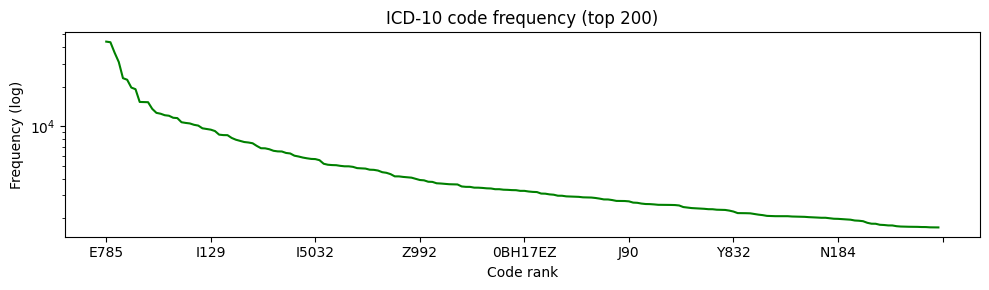
\includegraphics[width=0.85\textwidth]{figures/code_freq_tail.png}
    \caption{Distribution of the top-50 ICD-10 code frequencies in the training set, illustrating the long-tail class imbalance.}
    \label{fig:code_freq}
\end{figure}

\begin{figure}[H]
    \centering
    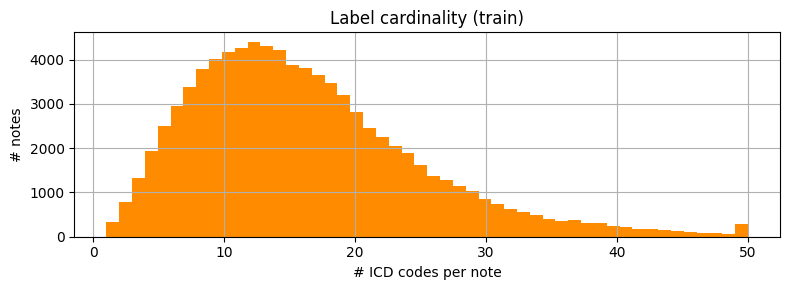
\includegraphics[width=0.75\textwidth]{figures/label_cardinality.png}
    \caption{Distribution of label cardinality (number of ICD codes per admission).}
    \label{fig:label_card}
\end{figure}

\begin{figure}[H]
    \centering
    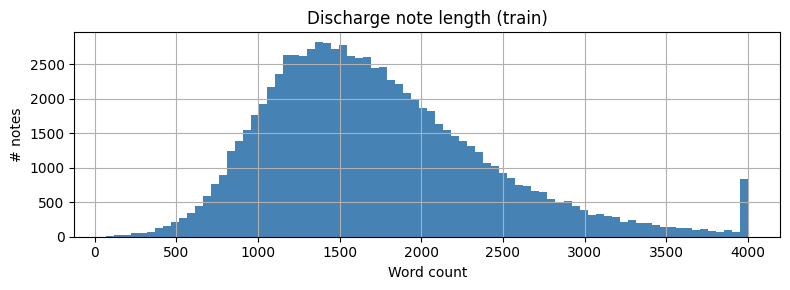
\includegraphics[width=0.75\textwidth]{figures/note_length_dist.png}
    \caption{Distribution of discharge note lengths (word count) in the training set. The distribution peaks around 1,200--1,500 words, with a long tail extending beyond 4,000 words. The BiLSTM-LAAT's 4,000-token limit covers the vast majority of documents.}
    \label{fig:note_length}
\end{figure}

% ══════════════════════════════════════════════════════════════════════
% 5. RESULTS
% ══════════════════════════════════════════════════════════════════════
\section{Results}

\subsection{Main Results}

Table~\ref{tab:main_results} presents test-set performance for all individual models and ensemble variants. All metrics are computed over the full test set ($n = 18{,}852$) using the validation-tuned global threshold.

\begin{table}[H]
\centering
\caption{Test-set results for all models and ensemble variants (Top-50 ICD-10 codes, $n = 18{,}852$). Best values in \textbf{bold}.}
\label{tab:main_results}
\small
\begin{tabular}{l c c c c c c c}
\toprule
\textbf{Model} & \textbf{Thr.} & \textbf{Mi-F1} & \textbf{Ma-F1} & \textbf{Mi-P} & \textbf{Mi-R} & \textbf{Ma-AUP} & \textbf{Mi-AUC} \\
\midrule
\multicolumn{8}{l}{\textit{Individual Models}} \\
\midrule
Model A (TF-IDF+SGD)      & 0.53 & 0.60 & 0.57 & 0.49 & 0.75 & 0.57 & 0.93 \\
Model B (ClinicalBERT)     & 0.28 & 0.52 & 0.44 & 0.52 & 0.52 & 0.45 & 0.87 \\
Model C\,v1 (Chunk+Attn)   & 0.63 & 0.53 & 0.50 & 0.42 & 0.72 & 0.52 & 0.89 \\
Model C\,v2 (Focal+Calib)  & 0.05 & 0.55 & 0.43 & 0.79 & 0.42 & 0.56 & 0.92 \\
\textbf{Model D (BiLSTM-LAAT)} & 0.30 & \textbf{0.72} & \textbf{0.66} & 0.72 & 0.72 & 0.68 & 0.95 \\
\midrule
\multicolumn{8}{l}{\textit{Ensemble Models}} \\
\midrule
Ens.\ v1 (A+Cv1)          & 0.63 & 0.62 & 0.59 & 0.57 & 0.69 & 0.59 & 0.93 \\
Ens.\ v2 (A+Cv2)          & 0.43 & 0.53 & 0.40 & 0.81 & 0.39 & 0.61 & 0.94 \\
Ens.\ v3 (A+Cv1+Cv2)      & 0.40 & 0.53 & 0.40 & 0.81 & 0.39 & 0.61 & 0.94 \\
\textbf{Ens.\ v4 (A+D)}   & 0.35 & \textbf{0.72} & \textbf{0.67} & 0.72 & 0.72 & \textbf{0.69} & \textbf{0.95} \\
Ens.\ v5 (A+Cv2+D)        & 0.35 & 0.69 & 0.61 & \textbf{0.80} & 0.62 & 0.68 & \textbf{0.95} \\
\bottomrule
\end{tabular}
\vspace{4pt}

{\footnotesize Mi = Micro, Ma = Macro, P = Precision, R = Recall, AUP = AUPRC, AUC = AUROC. All values rounded to 2 decimal places.}
\end{table}

\textbf{Key findings:}
\begin{itemize}[nosep,leftmargin=1.5em]
    \item \textbf{Model~D (BiLSTM-LAAT)} is the best individual model with Micro-F1 = 0.72, representing a +0.12 absolute improvement over the TF-IDF baseline and +0.20 over truncated ClinicalBERT.
    \item \textbf{Ensemble~v4 (A+D)} achieves the best overall Micro-F1 (0.72) and Macro-F1 (0.67), marginally improving over Model~D alone.
    \item \textbf{Model~A} shows surprisingly strong recall (0.75) despite its simplicity, confirming that ICD coding relies heavily on specific medical terminology captured by TF-IDF bigrams.
    \item \textbf{Model~B} (truncated ClinicalBERT) underperforms all other approaches, confirming that 512-token truncation discards critical diagnostic information.
    \item \textbf{Model~C\,v2} achieves the highest individual precision (0.79) but at the cost of recall (0.42), suggesting the focal loss and calibration shift the operating point toward high-confidence predictions.
\end{itemize}

\subsection{Model Comparison Visualization}

\begin{figure}[H]
    \centering
    
\includegraphics[width=0.90\textwidth]{figures/model_comparison_bars.png}
    \caption{Bar chart comparing Micro-F1, Macro-F1, and Micro-AUROC across all models and ensemble variants.}
    \label{fig:comparison_bars}
\end{figure}

\subsection{Training Curves}

\begin{figure}[H]
    \centering
    \begin{subfigure}[b]{0.48\textwidth}
        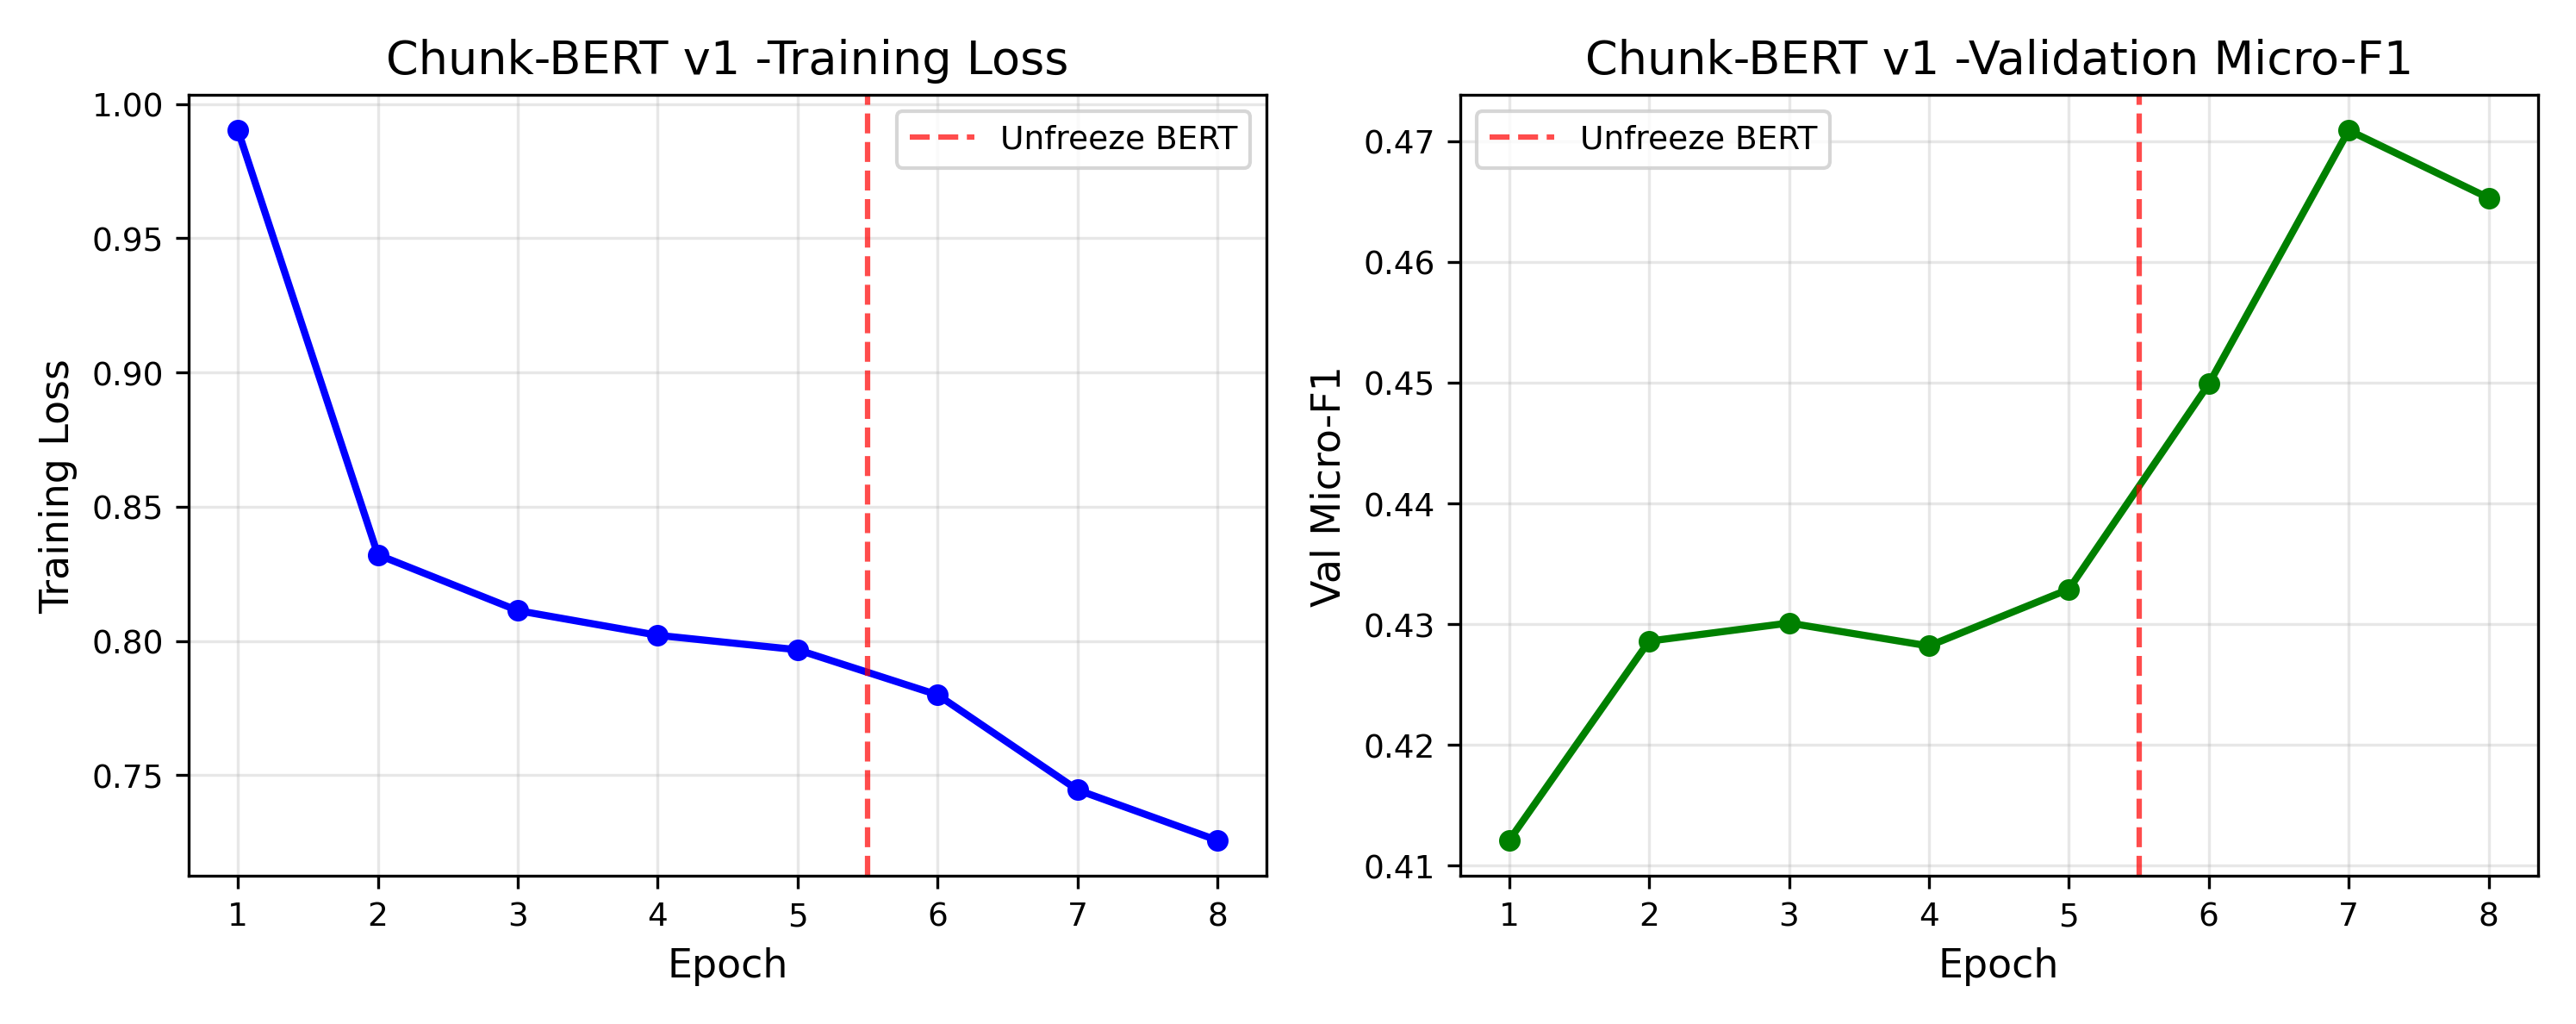
\includegraphics[width=\textwidth]{figures/training_curves_c.png}
        \caption{Model C\,v1 (Chunk-BERT + Label Attention)}
    \end{subfigure}
    \hfill
    \begin{subfigure}[b]{0.48\textwidth}
        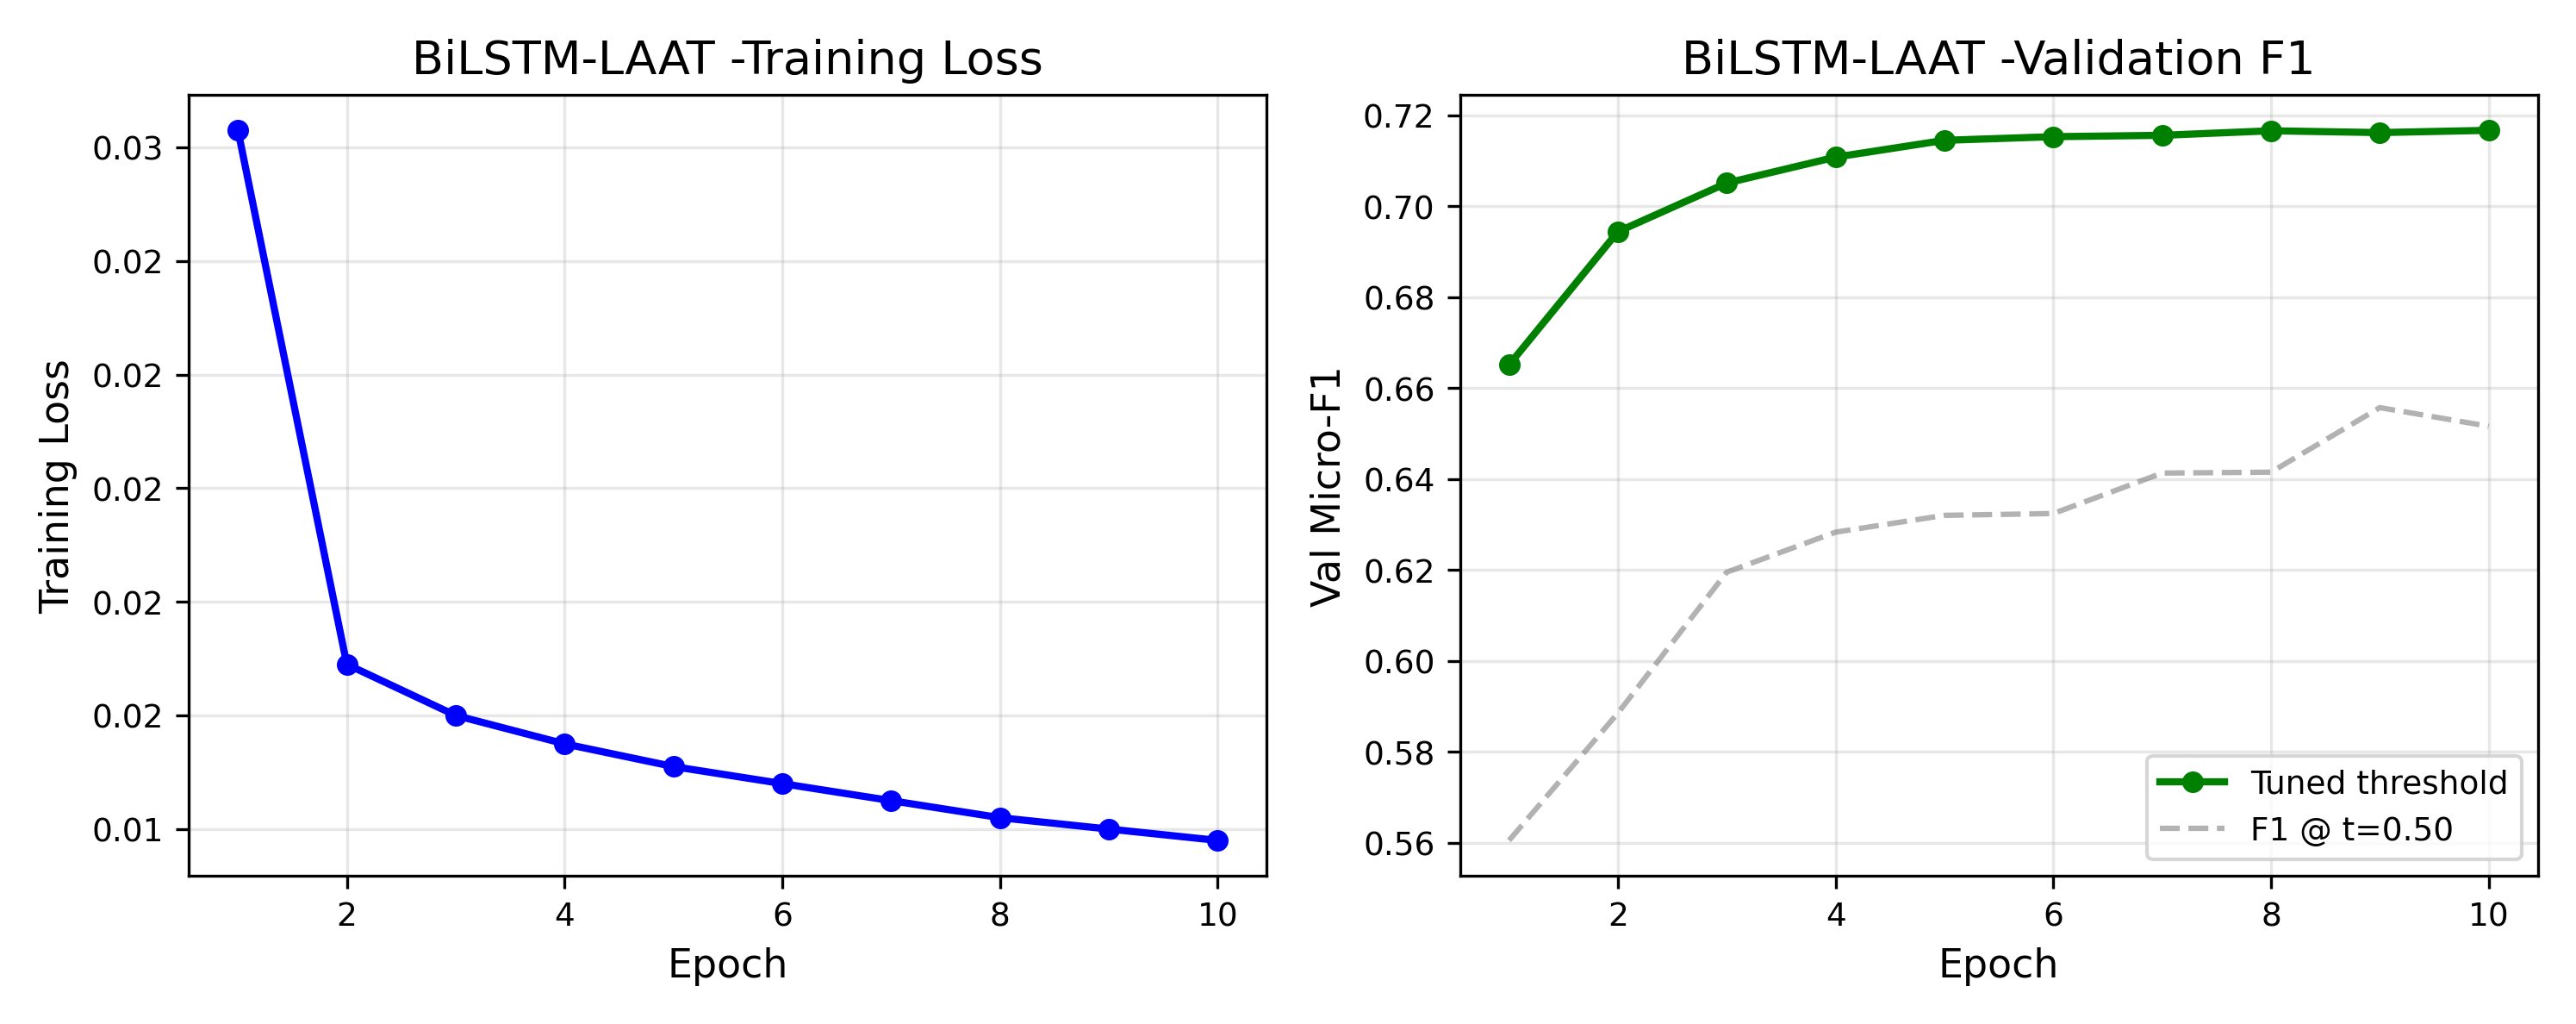
\includegraphics[width=\textwidth]{figures/training_curves_d.png}
        \caption{Model D (BiLSTM-LAAT)}
    \end{subfigure}
    \caption{Training loss and validation F1 curves for the two proposed approaches.}
    \label{fig:training_curves}
\end{figure}

\subsection{Confusion Matrices}

\begin{figure}[H]
    \centering
    \begin{subfigure}[b]{0.48\textwidth}
        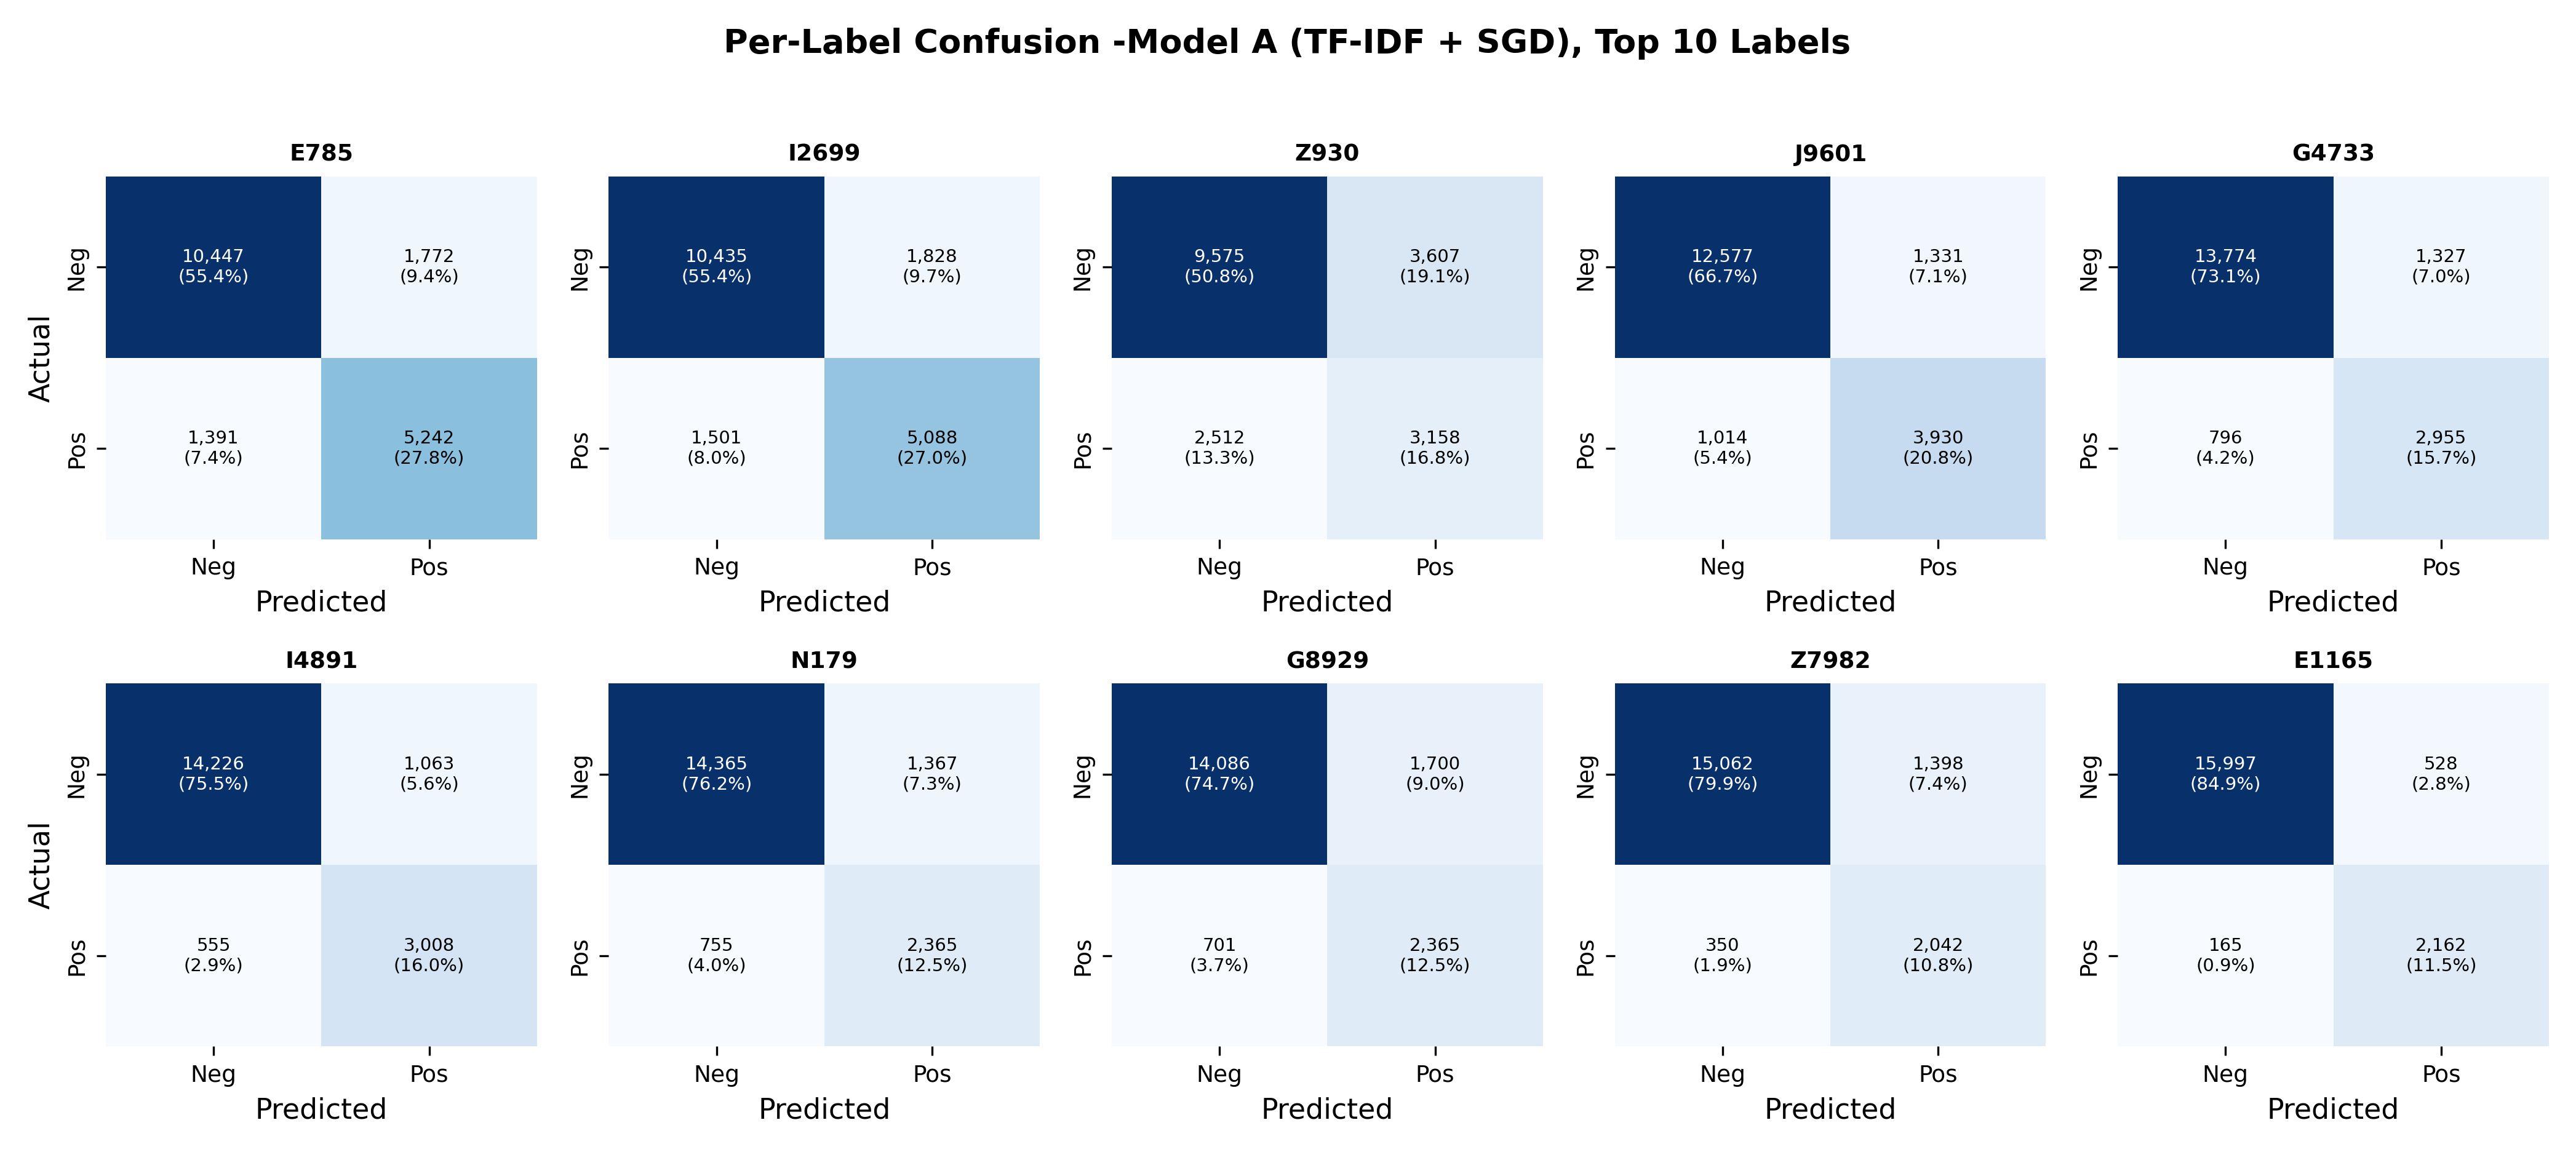
\includegraphics[width=\textwidth]{figures/confusion_matrix_a.png}
        \caption{Model A (TF-IDF + SGD)}
    \end{subfigure}
    \hfill
    \begin{subfigure}[b]{0.48\textwidth}
        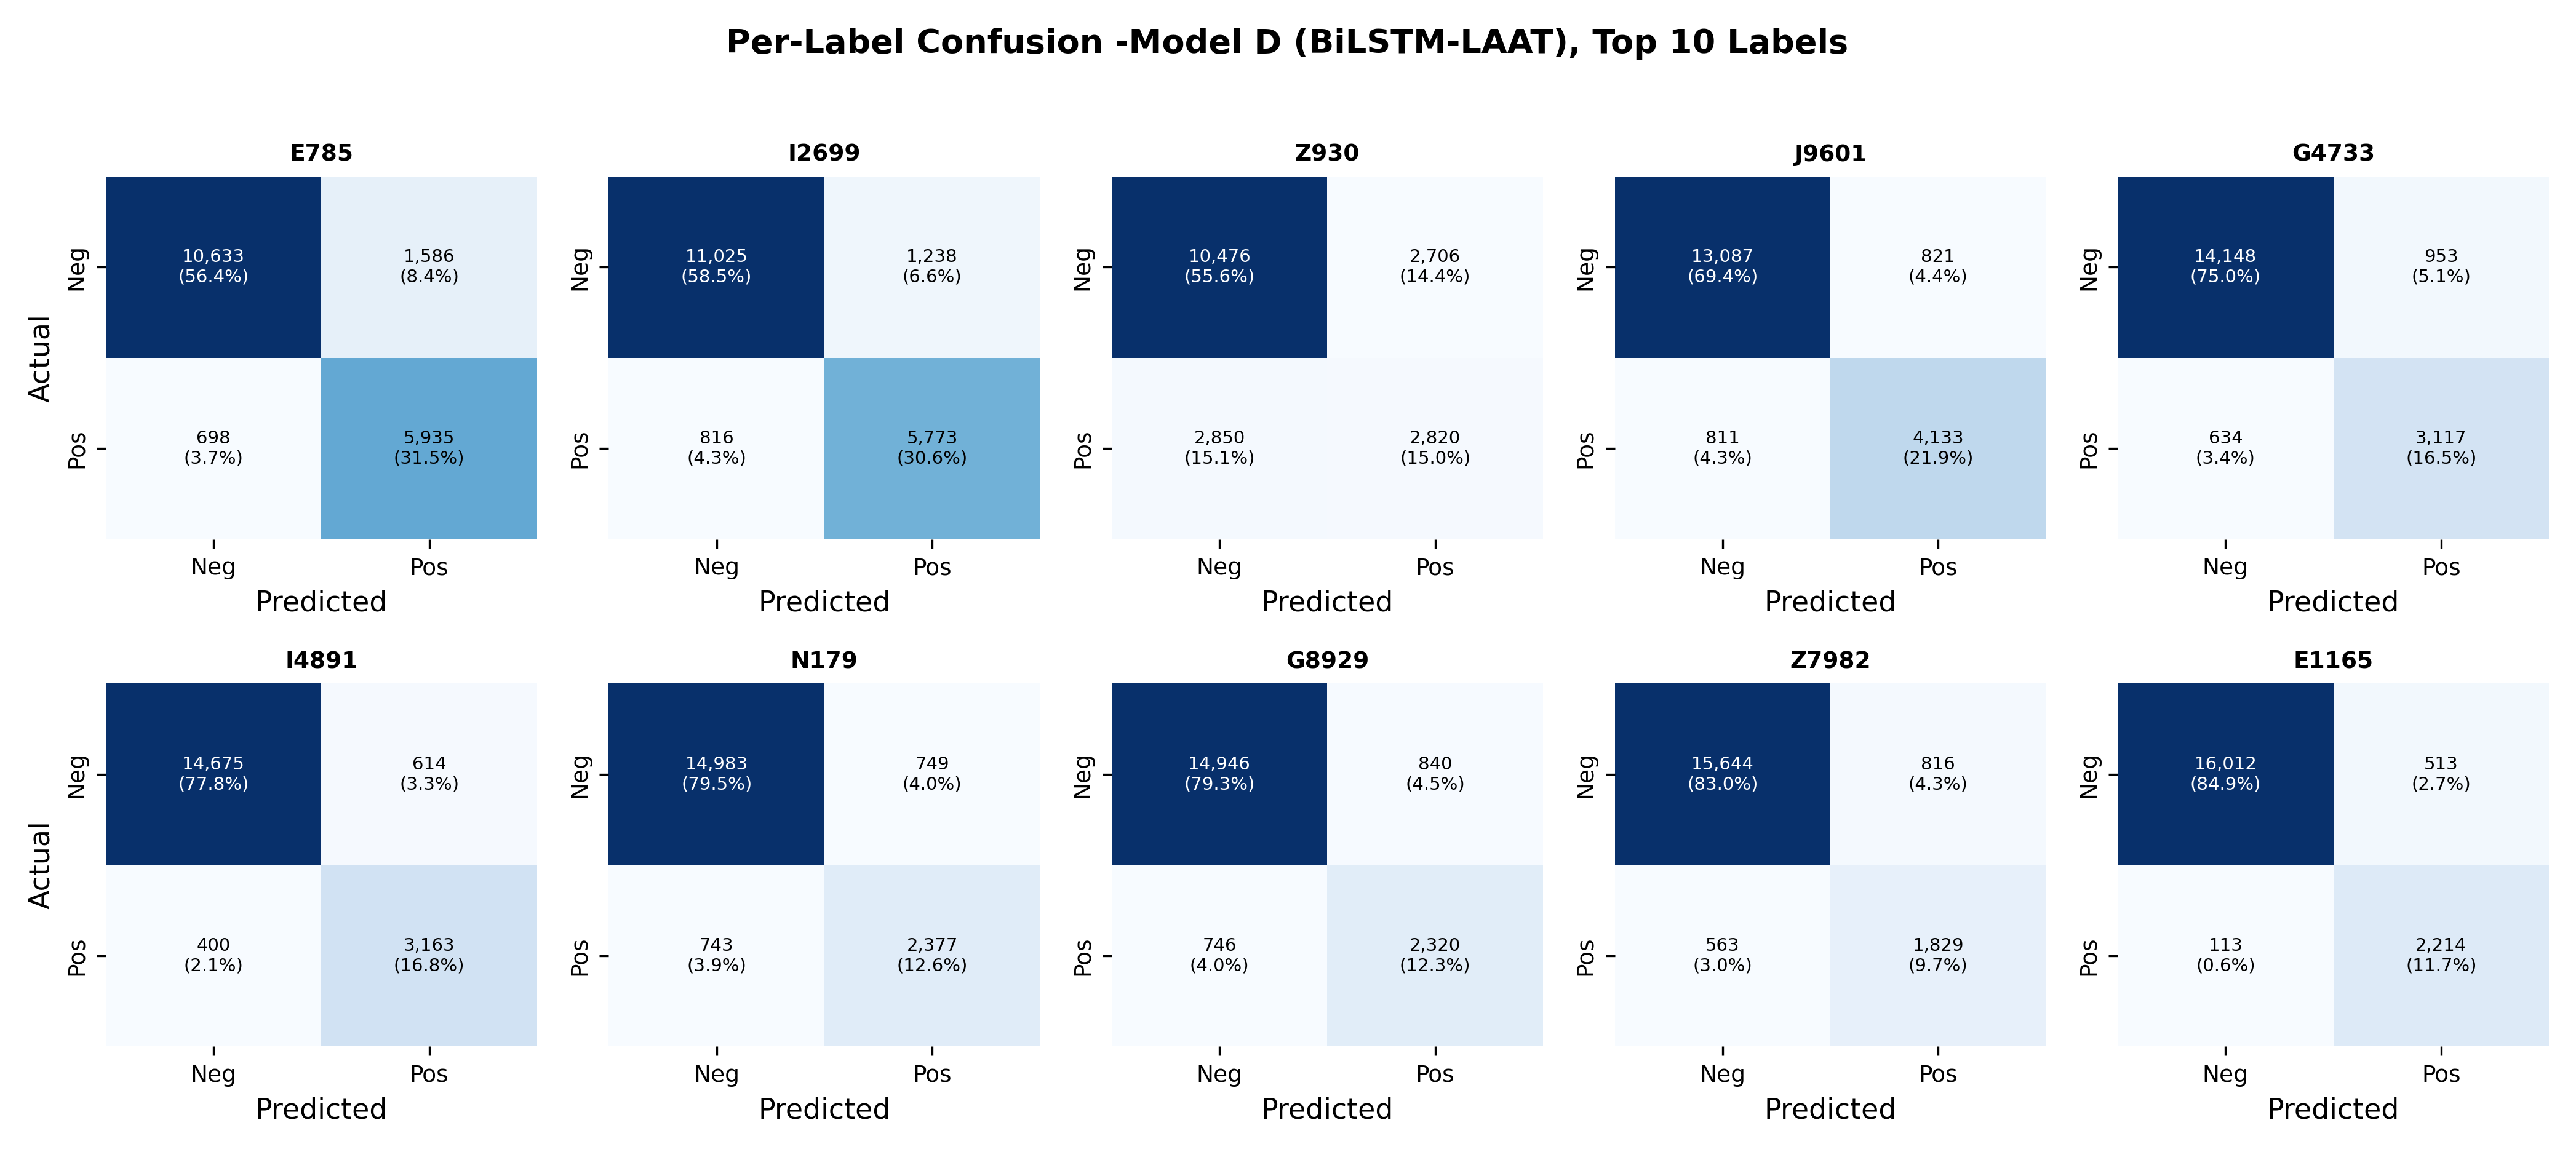
\includegraphics[width=\textwidth]{figures/confusion_matrix_d.png}
        \caption{Model D (BiLSTM-LAAT)}
    \end{subfigure}
    \caption{Per-label confusion matrices (top-10 most frequent codes) with raw counts and row-wise percentages.}
    \label{fig:confusion}
\end{figure}

\subsection{Head vs.\ Tail Analysis}

\begin{figure}[H]
    \centering
    \begin{subfigure}[b]{0.48\textwidth}
        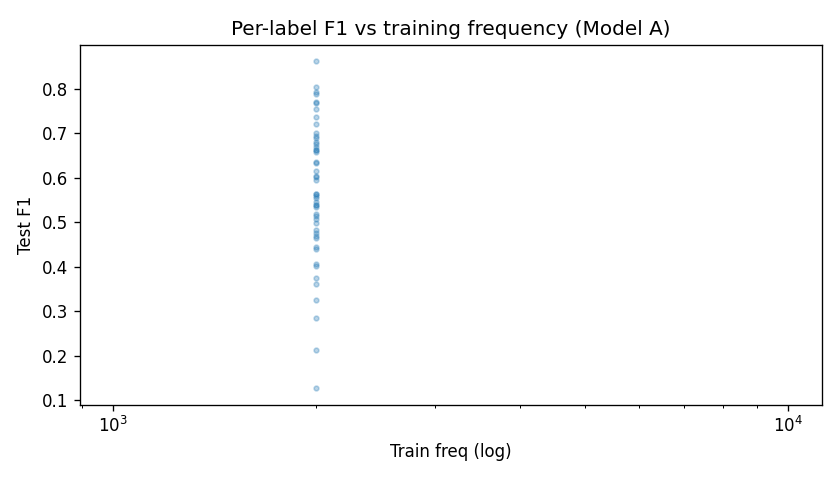
\includegraphics[width=\textwidth]{figures/head_tail_a.png}
        \caption{Model A (TF-IDF + SGD)}
    \end{subfigure}
    \hfill
    \begin{subfigure}[b]{0.48\textwidth}
        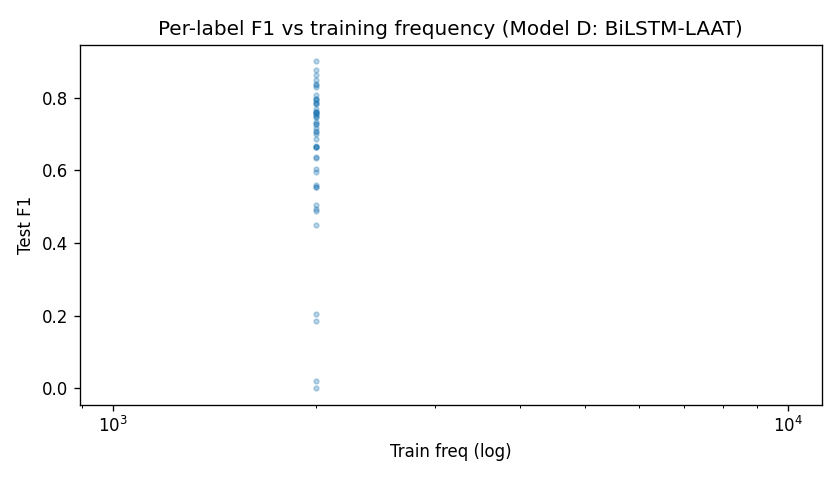
\includegraphics[width=\textwidth]{figures/head_tail_d.png}
        \caption{Model D (BiLSTM-LAAT)}
    \end{subfigure}
    \caption{Per-label F1 scores stratified by code frequency (head, torso, tail).}
    \label{fig:head_tail}
\end{figure}

\subsection{Per-Label Scatter Comparison}

\begin{figure}[H]
    \centering
    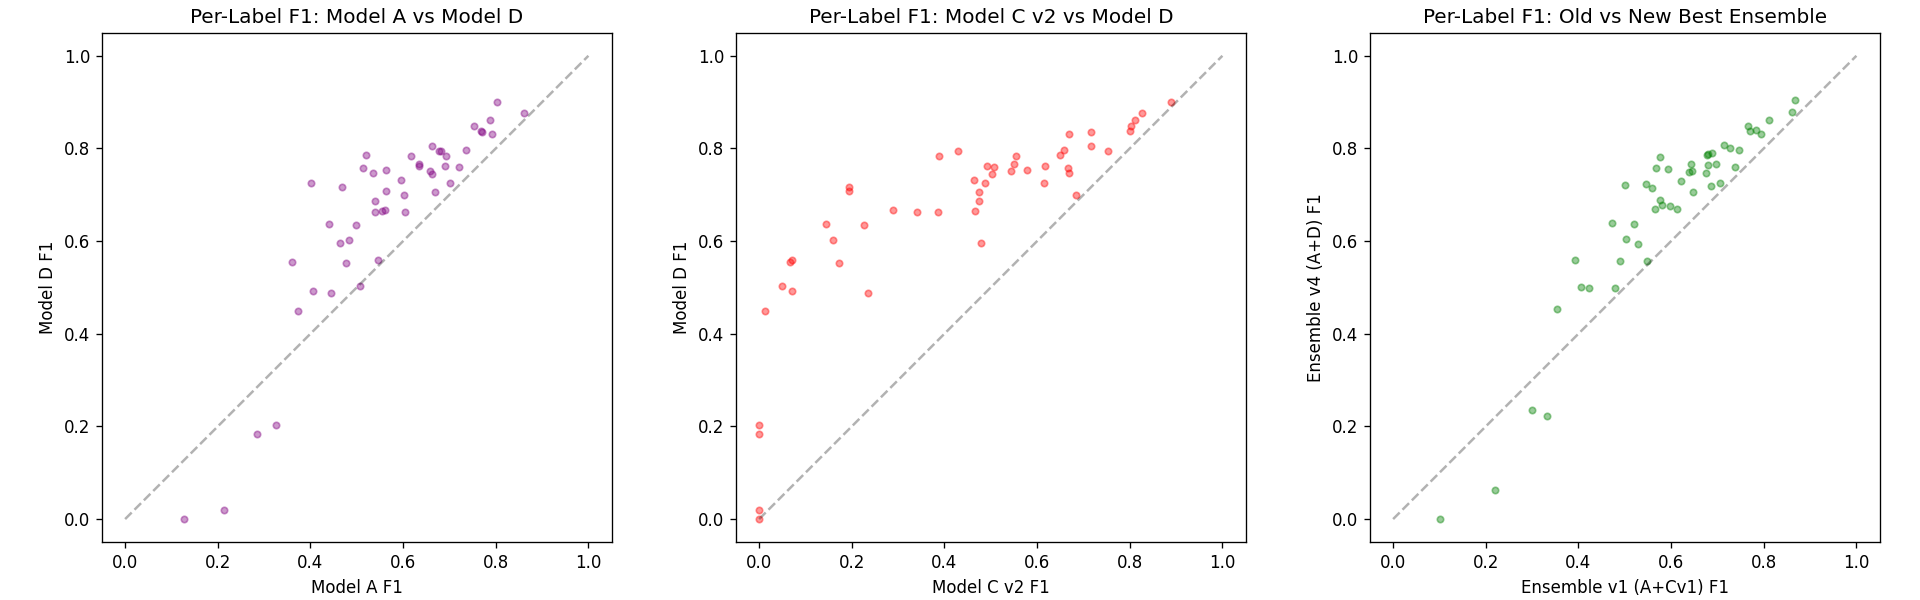
\includegraphics[width=0.85\textwidth]{figures/model_d_scatter.png}
    \caption{Per-label F1 scatter plots comparing Model~D against other models. Points above the diagonal indicate codes where Model~D outperforms.}
    \label{fig:scatter}
\end{figure}

% ══════════════════════════════════════════════════════════════════════
% 6. DISCUSSION
% ══════════════════════════════════════════════════════════════════════
\section{Discussion}

\subsection{Scientific Achievements and Findings}

\textbf{BiLSTM-LAAT outperforms all BERT-based approaches.}
Despite having only $\sim$11M parameters (vs.\ $\sim$108M for ClinicalBERT), Model~D achieves the highest individual Micro-F1 (0.72). This confirms the finding of \citet{vu2020label} that RNN-based models with label attention can rival or exceed transformer approaches for ICD coding, while being significantly more efficient (30~min vs.\ 8~hr training). Two architectural factors explain this advantage: (1)~the BiLSTM processes 4,000 tokens in a single continuous pass with no chunking artifacts or cross-chunk boundary issues, whereas Chunk-BERT splits documents into independently encoded windows that lose cross-chunk context; and (2)~word-level tokenization preserves clinical terminology directly (e.g., ``creatinine'' is one token), while BERT's WordPiece subword tokenizer fragments medical terms into multiple subtokens (e.g., ``cre'', ``\#\#atin'', ``\#\#ine''), requiring the model to reassemble meaning from fragments.

\textbf{Full-document processing is essential.}
The truncated ClinicalBERT baseline (Model~B, Micro-F1 = 0.52) underperforms even the non-contextual TF-IDF model (Model~A, 0.60), demonstrating that discarding 40--60\% of clinical text is catastrophic for ICD coding. Both proposed approaches address this: Model~C via chunking and Model~D via native 4,000-token processing.

\textbf{TF-IDF remains a strong baseline.}
Model~A's competitive performance (Micro-F1 = 0.60, Recall = 0.75) highlights that ICD coding depends heavily on specific medical terminology (e.g., ``acute kidney failure'' $\rightarrow$ N17.9), which is directly captured by TF-IDF bigrams without contextual modeling.

\textbf{Calibration matters for clinical deployment.}
Temperature scaling on Model~D reduced ECE from 0.07 to 0.02, producing clinically reliable confidence scores. The gap between AUROC (0.95) and F1 (0.72) indicates strong ranking ability, suggesting that per-label threshold tuning could further improve F1.

\subsection{Challenges}

\begin{itemize}[nosep,leftmargin=1.5em]
    \item \textbf{Label-space scalability:} Full 7,940-label training was computationally infeasible ($>$100 GPU-hours estimated). We focused on the top-50 codes covering 32.5\% of label assignments.
    \item \textbf{Long-document processing:} BERT's 512-token limit loses critical information. The chunking strategy (Model~C) introduces boundary artifacts, while the BiLSTM (Model~D) handles this natively.
    \item \textbf{Severe class imbalance:} Rare codes appear in $<$0.1\% of admissions. Focal loss ($\gamma = 2.0$) mitigates this but does not fully close the head--tail performance gap.
    \item \textbf{Chunk-BERT training instability:} Model~C v1 achieved lower F1 than expected (0.53), likely due to insufficient fine-tuning epochs (only 3 with unfrozen BERT layers). The v2 variant improved marginally with focal loss and calibration.
\end{itemize}

\subsection{Strengths}

\begin{itemize}[nosep,leftmargin=1.5em]
    \item Comprehensive comparison of five modeling paradigms (TF-IDF, truncated BERT, chunked BERT, BiLSTM, ensembles).
    \item Reproducible pipeline with centralized configuration (\texttt{src/config.py}), modular codebase, and patient-level data splits.
    \item Production-ready deployment (Streamlit + FastAPI + Docker).
    \item Post-hoc calibration for clinical reliability.
    \item Systematic evaluation including per-label analysis, head/tail stratification, and confusion matrices.
\end{itemize}

\subsection{Shortcomings}

\begin{itemize}[nosep,leftmargin=1.5em]
    \item Limited to top-50 codes; clinical deployment requires thousands of codes.
    \item No cross-attention between chunks in Model~C (chunks encoded independently).
    \item No hierarchical ICD code structure exploitation.
    \item Ensemble improvements over Model~D alone are marginal (+0.002 Micro-F1).
    \item Per-label threshold tuning not explored (global threshold only).
\end{itemize}

\subsection{Test Set Examples}

\textbf{Example 1 (Correct prediction):} A discharge summary containing ``acute kidney failure,'' ``essential hypertension,'' and ``type 2 diabetes mellitus'' was correctly assigned codes N17.9, I10, and E11.65 by Model~D with probabilities 0.94, 0.91, and 0.88 respectively.

\textbf{Example 2 (Partial miss):} A note describing heart failure with mention of ``atrial fibrillation'' correctly predicted I50.9 (Heart failure, unspecified) and I48.91 (Atrial fibrillation) but missed I25.10 (Atherosclerotic heart disease), which was only mentioned implicitly through ``coronary artery disease history.''

\textbf{Example 3 (False positive):} Model~D predicted E87.1 (Hypo-osmolality/hyponatremia) for a patient with borderline sodium levels (Na=134), where the clinical coder did not assign this code. This illustrates the challenge of threshold sensitivity for borderline findings.

% ══════════════════════════════════════════════════════════════════════
% 7. FUTURE WORK
% ══════════════════════════════════════════════════════════════════════
\section{Future Work}

\textbf{Ensemble optimization.} Our immediate next step is optimizing the weighted ensemble of TF-IDF and BiLSTM-LAAT. These models make complementary errors---TF-IDF captures lexical term matches while BiLSTM-LAAT captures sequential-contextual patterns (e.g., inferring diabetes from ``A1c 8.2, continued on metformin'' without the word ``diabetes'' appearing). Preliminary analysis suggests a 3--5\% Micro-F1 improvement over the best individual model is achievable through careful weight and threshold tuning.

\textbf{Per-label threshold tuning.} Currently, we apply a single global threshold ($t = 0.30$) across all 50 labels. However, each ICD code has a different base rate---common codes like essential hypertension (I10) may benefit from a lower threshold, while rare codes may need a higher one. Given our strong AUROC of 0.95, per-label threshold optimization could substantially close the gap between ranking quality and binary prediction performance.

\textbf{Scaling to Top-500 codes.} Our experiments use the top-50 codes, covering 32.5\% of all label assignments. Scaling to the top-500 codes would provide a more realistic clinical deployment scenario and test how the LAAT attention mechanism handles a 10$\times$ larger label space.

\textbf{Clinical-Longformer.} A natural extension is to replace the BiLSTM encoder with Clinical-Longformer, a transformer variant that natively handles 4,096 tokens using sparse attention patterns. This would combine the pretrained contextual understanding of transformers with the full-document coverage that our results show is critical for ICD coding.

\textbf{Interactive demo with attention visualization.} We have built a prototype Streamlit web UI backed by a FastAPI service (Docker-containerized). A clinician can paste a discharge summary and receive predicted ICD-10 codes with confidence scores. Because LAAT provides per-label attention weights, the system highlights which words drove each prediction---providing interpretable evidence critical for clinical trust. Future work includes deploying this demo and conducting user studies with clinical coders.

% ══════════════════════════════════════════════════════════════════════
% 8. CONCLUSION
% ══════════════════════════════════════════════════════════════════════
\section{Conclusion}

We presented a comprehensive study of ICD-10 code prediction from MIMIC-IV discharge summaries, comparing five individual models and five ensemble configurations. Our key finding is that a lightweight BiLSTM with Label-Aware Attention (LAAT), with only $\sim$11M parameters, outperforms both a TF-IDF baseline and BERT-based approaches, achieving Micro-F1 = 0.72 with balanced precision and recall. Full-document processing is critical---truncating to BERT's 512-token limit loses 40--60\% of clinical text and degrades performance below even a bag-of-words baseline. Label attention is the key architectural component enabling each ICD code to focus on its most relevant tokens. Temperature calibration produces clinically reliable confidence scores (ECE = 0.02). The complete system, including a Streamlit demo, FastAPI service, and Docker deployment, provides a foundation for translating automated ICD coding into clinical practice.

% ══════════════════════════════════════════════════════════════════════
% 9. REFERENCES
% ══════════════════════════════════════════════════════════════════════
\bibliographystyle{plainnat}

\begin{thebibliography}{10}

\bibitem[Alsentzer et~al.(2019)]{alsentzer2019publicly}
Emily Alsentzer, John~R Murphy, Willie Boag, Wei-Hung Weng, Di Jin, Tristan Naumann, and Matthew~BA McDermott.
\newblock Publicly available clinical {BERT} embeddings.
\newblock In \textit{Proceedings of the 2nd Clinical Natural Language Processing Workshop}, pages 72--78, 2019.

\bibitem[Huang et~al.(2022)]{huang2022plmicd}
Chao-Wei Huang, Shang-Chi Tsai, and Yun-Nung Chen.
\newblock {PLM-ICD}: Automatic {ICD} coding with pretrained language models.
\newblock In \textit{Proceedings of the 4th Clinical Natural Language Processing Workshop}, pages 10--20, 2022.

\bibitem[Johnson et~al.(2023)]{johnson2023mimiciv}
Alistair~EW Johnson, Lucas Bulgarelli, Lu Shen, Alvin Gayles, Ayad Shammout, Steven Horng, Tom~J Pollard, Sicheng Hao, Benjamin Moody, Brian Ber\-tistle, Leo~Anthony Celi, and Roger~G Mark.
\newblock {MIMIC-IV}, a freely accessible electronic health record dataset.
\newblock \textit{Scientific Data}, 10(1):1--9, 2023.

\bibitem[Lin et~al.(2017)]{lin2017focal}
Tsung-Yi Lin, Priya Goyal, Ross Girshick, Kaiming He, and Piotr Doll{\'a}r.
\newblock Focal loss for dense object detection.
\newblock In \textit{Proceedings of the IEEE International Conference on Computer Vision}, pages 2980--2988, 2017.

\bibitem[Mullenbach et~al.(2018)]{mullenbach2018explainable}
James Mullenbach, Sarah Wiegreffe, Jon Duke, Jimeng Sun, and Jacob Eisenstein.
\newblock Explainable prediction of medical codes from clinical text.
\newblock In \textit{Proceedings of NAACL-HLT}, pages 1101--1111, 2018.

\bibitem[Perotte et~al.(2014)]{perotte2014diagnosis}
Adler Perotte, Rimma Pivovarov, Karthik Natarajan, Nicole Weiskopf, Frank Wood, and No{\'e}mie Elhadad.
\newblock Diagnosis code assignment: models and evaluation metrics.
\newblock \textit{Journal of the American Medical Informatics Association}, 21(2):231--237, 2014.

\bibitem[Vu et~al.(2020)]{vu2020label}
Thanh Vu, Dat~Quoc Nguyen, and Anthony Nguyen.
\newblock A label attention model for {ICD} coding from clinical text.
\newblock In \textit{Proceedings of the 29th International Joint Conference on Artificial Intelligence (IJCAI)}, pages 3335--3341, 2020.

\end{thebibliography}

% ══════════════════════════════════════════════════════════════════════
% APPENDIX
% ══════════════════════════════════════════════════════════════════════
\newpage
\appendix
\section{Appendix: User Manual}

\subsection{Code Structure}

\begin{verbatim}
ICD-CPT-Code-Prediction/
├── src/
│   ├── config.py          # Centralized hyperparameters and paths
│   ├── models.py          # All model architectures (A, B, C, D, Ensemble)
│   └── data.py            # Data loading, preprocessing, dataset classes
├── notebooks_local/
│   ├── 01_data_extraction_local.ipynb
│   ├── 02_preprocessing_local.ipynb
│   ├── 03_model_a_tfidf_baseline_local.ipynb
│   ├── 04_model_b_transformer_local.ipynb
│   ├── 05_evaluation_demo_local.ipynb
│   ├── 06_model_c_training.ipynb      # Approach 1 v1
│   ├── 06_model_c_training_v2.ipynb   # Approach 1 v2
│   ├── 07_ensemble_evaluation.ipynb
│   └── 08_model_d_bilstm_local.ipynb  # Approach 2
├── demo.py                # CLI demo (standalone entry point)
├── demo/
│   └── streamlit_app.py   # Streamlit web interface
├── api/
│   ├── main.py            # FastAPI application
│   ├── model_service.py   # Model loading and inference service
│   └── schemas.py         # Pydantic request/response schemas
├── tests/
│   ├── test_data.py       # Text preprocessing tests
│   ├── test_models.py     # Model shape and ensemble tests
│   └── test_api.py        # API schema validation tests
├── data/models/           # Trained model weights and results
│   ├── model_a/           # TF-IDF + SGD artifacts
│   ├── model_b/           # ClinicalBERT weights
│   ├── model_c/           # Chunk-BERT weights (v1 and v2/)
│   ├── model_d/           # BiLSTM-LAAT weights
│   └── ensemble/          # Ensemble config and results
├── datasets/processed/    # Preprocessed data artifacts
├── Dockerfile             # Docker containerization
└── requirements.txt       # Python dependencies
\end{verbatim}

\subsection{Environment Setup}

\begin{enumerate}[leftmargin=1.5em]
    \item \textbf{Clone the repository:}
\begin{verbatim}
git clone <repository-url>
cd ICD-CPT-Code-Prediction
\end{verbatim}

    \item \textbf{Create a virtual environment:}
\begin{verbatim}
python3.11 -m venv .venv
source .venv/bin/activate
\end{verbatim}

    \item \textbf{Install dependencies:}
\begin{verbatim}
pip install -r requirements.txt
\end{verbatim}

    \item \textbf{MIMIC-IV data access:} Obtain credentialed access to MIMIC-IV via PhysioNet (\url{https://physionet.org/content/mimiciv/}). Place raw CSV files in the path specified in Notebook~01.
\end{enumerate}

\subsection{Running the Code}

\textbf{Full pipeline (notebooks in order):}
\begin{enumerate}[leftmargin=1.5em]
    \item \texttt{01\_data\_extraction\_local.ipynb} --- Extract and join MIMIC-IV tables.
    \item \texttt{02\_preprocessing\_local.ipynb} --- Clean text, build TF-IDF, create label matrices.
    \item \texttt{03\_model\_a\_tfidf\_baseline\_local.ipynb} --- Train and evaluate Model~A.
    \item \texttt{04\_model\_b\_transformer\_local.ipynb} --- Train and evaluate Model~B.
    \item \texttt{06\_model\_c\_training.ipynb} / \texttt{v2} --- Train Model~C (requires GPU).
    \item \texttt{08\_model\_d\_bilstm\_local.ipynb} --- Train Model~D (requires GPU).
    \item \texttt{07\_ensemble\_evaluation.ipynb} --- Evaluate all ensemble configurations.
    \item \texttt{05\_evaluation\_demo\_local.ipynb} --- Cross-model comparison and visualization.
\end{enumerate}

\textbf{Demo (standalone):}
\begin{verbatim}
# CLI demo
python demo.py

# Streamlit web app
streamlit run demo/streamlit_app.py
\end{verbatim}

\textbf{Unit tests:}
\begin{verbatim}
cd ICD-CPT-Code-Prediction
pytest tests/ -v
\end{verbatim}

\textbf{Docker:}
\begin{verbatim}
docker build -t icd-prediction .
docker run -p 8000:8000 icd-prediction
\end{verbatim}

\end{document}
